Dans ce chapitre, nous explorons la notion de type dans les langages de
programmation. Tout d'abord pourquoi elle existe et en quoi elle aide à rendre
les programmes plus sûrs. Il y a autant de système de types que de langages de
programmation, donc nous présenterons ensuite une taxonomie de ces systèmes en
les regroupant par caractéristiques communes. Cette classification sera appuyée
par des exemples de code C\cite{AnsiC,KandR},
OCaml\link{ocamlManual}\cite{DAOC}, Haskell\link{haskell}\cite{haskell98,rwh},
Python\link{python} et Perl\link{perl}\cite{perlCamelBook}.

\section{Présentation et but}

\section{Taxonomie}

\subsection{Dynamique, statique, mixte}

A première vue, cela semble moins puissant que le typage dynamique : en effet,
il existe des programmes qui s'exécuteront sans erreur de type mais sur lesquels
le typage statique ne peut s'appliquer. Dans la figure~\ref{fig:nontypable}, on
peut voir par une simple analyse de cas que si on fournit un booléen à
\texttt{f}, elle retourne un entier. Mais selon la valeur de \texttt{b}, la
variable \texttt{x} contiendra une valeur de type entier ou fonction.

\subsection{Fort, faible, sound}

\begin{figure}
  \insertcode{cast.java}
  \caption{Transtypage en Java}
  \label{fig:javacast}
\end{figure}

Si un système de types statique permet d'éliminer totalement la nécessité de
réaliser des tests de typage, on dit qu'il est \emph{fort}. Mais ce n'est que
rarement le cas. En effet, il peut y avoir des constructions au sein du langage
qui permettent de contourner le système de types, comme un opérateur de
transtypage\ref{fig:javacast}. À l'exécution, une erreur de types est levée :

\begin{Verbatim}
Exception in thread "main" java.lang.ClassCastException:
    java.lang.Integer cannot be cast to java.lang.Float
        at Cast.main(Cast.java:5)
\end{Verbatim}

\clearpage

\wip{}


\begin{figure}
\centering
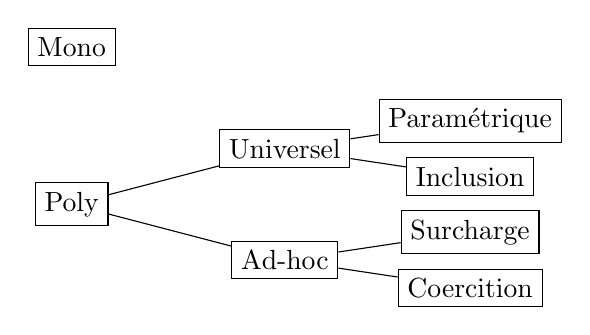
\begin{tikzpicture}
  [ ptype/.style={draw=black,shape=rectangle}
  , child/.style={ptype, xshift=2cm}
  , gen0/.style={       node distance=2cm}
  , gen1/.style={child, node distance=1cm}
  , gen2/.style={child, node distance=5mm}
  ]

  \node[ptype]                     (mono) {Mono};
  \node[ptype,below of=mono, gen0] (poly) {Poly};
  \node[above right of=poly, gen1] (univ)  {Universel};
  \node[above right of=univ, gen2] (param) {Paramétrique};
  \node[below right of=univ, gen2] (inclu) {Inclusion};
  \node[below right of=poly, gen1] (adho)  {Ad-hoc};
  \node[above right of=adho, gen2] (over)  {Surcharge};
  \node[below right of=adho, gen2] (coer)  {Coercition};

  \draw (poly) -- (univ);
  \draw (poly) -- (adho);

  \draw (univ) -- (param);
  \draw (univ) -- (inclu);

  \draw (adho) -- (over);
  \draw (adho) -- (coer);

      %node {Mono}
      %node {Poly}
          %node {Universal}
              %node {Param}
              %node {Inclusion}
          %node {Ad-Hoc}
              %node {Surcharge}
              %node {Coercition}

\end{tikzpicture}

\caption{Les différents types de polymorphisme.}
\label{fig:types-de-polymorphisme}
\end{figure}


\subsubsection{Polymorphisme universel}

% = {paramétrique, par inclusion}

Le polymorphisme est dit universel si toute fonction générique peut s'appliquer
à n'importe quel type.

\subsubsection{Polymorphisme ad-hoc}

% = {par surcharge, par coercition}

Le polymorphisme est \emph{ad-hoc} si les fonctions génériques ne peuvent
s'appliquer qu'à un ensemble de types prédéfini.

\subsubsection{Polymorphisme par sous-typage}

\todo{héritage,sous-typage,classe,méthode,héritage multiple,late binding,Liskov}

Certains langages définissent la notion de sous-typage. C'est une relation
d'ordre partiel sur les types, qui modélise la relation "est un". Chaque
sous-classe peut redéfinir le comportement de chaque méthode de ses
superclasses.

\subsubsection{Polymorphisme par surcharge}

Considérons l'opération d'addition : \texttt{+}. On peut considérer que certains
types l'implémentent, et pas d'autres : ajouter deux flottants ou deux entiers a
du sens, mais pas ajouter deux pointeurs.

On dira que \texttt{+} est \emph{surchargé}. À chaque site d'appel, il faudra
\emph{résoudre la surcharge} pour déterminer quelle fonction appeler.

Cela rend l'inférence de types \todo{introduire l'inférence plus haut}
impossible dans le cas général, puisque certaines constructions sont ambigües.

\begin{figure}
  \insertcode{showread.hs}
  \caption{Cas d'ambigüité avec de la surcharge ad-hoc.}
  \label{fig:showread}
\end{figure}

Dans le code Haskell de la figure~\ref{fig:showread}, \texttt{show} peut
s'appliquer à toutes les valeurs de types "affichables" et renvoie une
représentation textuelle. \texttt{read} réalise le contraire avec les types
"lisibles".

Lorsqu'on compose ces deux fonctions, le type de la valeur intermédiaire est
capital puisqu'il détermine les instances de \texttt{show} et \texttt{read} à
utiliser.

\subsubsection{Polymorphisme par coercition}

\subsubsection{Polymorphisme d'ordre supérieur}

\begin{verbatim}
g f = (f true, f 2)
\end{verbatim}

\[
g : (\forall a . a -> a) -> (bool * int)
\]

Pas inférable (annotations nécessaires).

\subsection{Expressivité, garanties, types dépendants}

\section{Exemples}

\subsection{Faible dynamique : Perl}
\subsection{Faible statique : C}
\subsection{Fort dynamique : Python}
\subsection{Fort statique : OCaml}
\subsection{Fort statique à effets typés : Haskell}
\subsection{Theorem prover : Coq}

% vim: spelllang=fr
